\section{Datasets}
\label{sec:db}

The annotated segmentation, saliency, object and scenes classification datasets, which are produced and used by the researchers to test the algorithms are often made available to the community.

\subsection{Image Saliency Datasets}
\subsubsection{MSRA}\label{subsec:msra}
The MSRA  Database form the Visual computing group of Microsoft Research Asia \cite{msra_db} is  first large-scale labeled dataset made publically available for training and evaluation. It contains two image sets. The first set consists of $20 000$ images labeled by three users, while the second set consists of $5000$ images labeled by nine users. The labeling are available as bounding boxes. Figure \ref{fig:msra} illustrates the dataset.
\begin{figure}[H]
\begin{center}
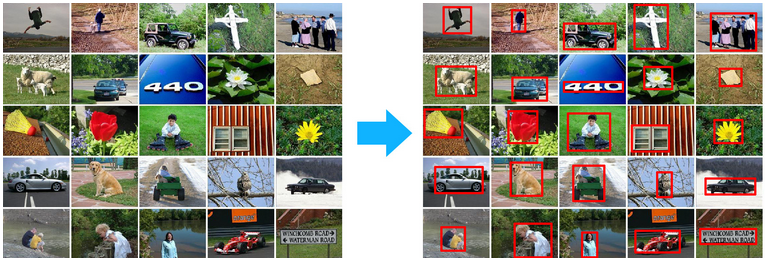
\includegraphics[width=0.95\textwidth]{fig/MSRA}
\end{center}
\caption{Examples of the MSRA dataset.}
\label{fig:msra}
\end{figure}

The results of the proposed method by the authors of the dataset, have been published in \cite{LiuCVPR2007}.

\subsubsection{MSRA10k}
This is an extension of the MSRA dataset, which  addresses the coarse-grained limitation of the MSRA labeling (bounding boxes). The MSRA10k (\cite{msra10k_db}) dataset consists of $10000$ randomly selected MSRA images for which a pixel-level saliency labeling is available. Figure \ref{fig:msra10k} illustrates the dataset. 
\begin{figure}[H]
\begin{center}
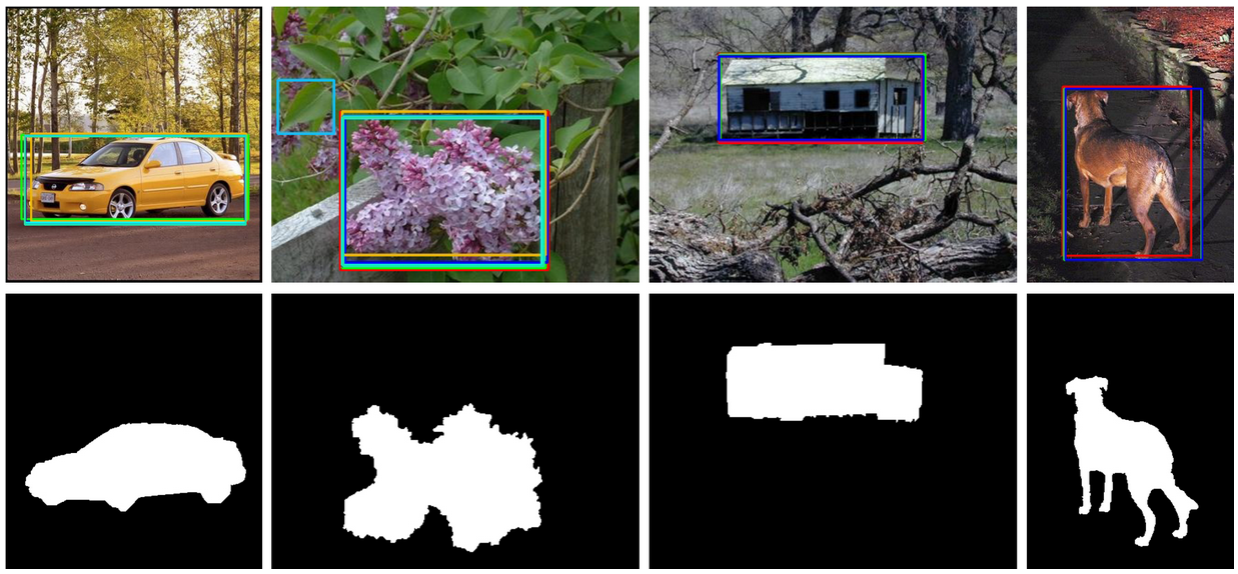
\includegraphics[width=0.95\textwidth]{fig/MSRA10k}
\end{center}
\caption{Examples of the MSRA 10k dataset. First row: original images with ground truth rectangles from MSRA dataset. Second row: Ground truth with pixel accuracy.}
\label{fig:msra10k}
\end{figure}
This dataset is used by in a very recent paper in IEEE Transactions on PAMI \cite{ChengPAMI2015} and \cite{chengPAMIUrl} (online resources with link to the software). 

\subsubsection{CSSD and ECSSD}\label{subsec:cssd}
Although images from MSRA-1000 \cite{LCAV-CONF-2009-012} have a large variety in their content, background structures are primarily simple and smooth. To represent the situations that natural images generally fall into, the Complex Scene Saliency Dataset (CSSD) \cite{cssd_db} was proposed in \cite{YanCVPR2013} with $200$ images. They contain diverse patterns in both foreground and background. The labeling has done by five  helpers. These images were collected from the BSD300 (later extended to BSD500, \cite{bsd300/500_db}), VOC dataset \cite{voc_db} and internet.

Later, the CSSD was extended to a larger dataset (ECSSD) of $1000$ images, which includes many semantically meaningful and structurally complex images for evaluation. The images are acquired from the internet and five helpers were asked to produce the ground truth masks. Examples of the images in the dataset can be seen on Figure \ref{fig:ecssd}.

\begin{figure}[h]
\begin{center}
\includegraphics[width=0.95\textwidth]{fig/ECSSD}
\end{center}
\caption{Examples of the ECSSD dataset.}
\label{fig:ecssd}
\end{figure}

\subsubsection{DUT-OMRON}
The Dalian University of Technology and the Omron Corporation introduced in the DUT-OMRON dataset \cite{dut-omron_db} consisting of $5168$, manually selected from more than $140 000$ images. They are re-sized to $400 \times x$ or $x \times 400$, where  $x < 400$. They contain one or more salient objects with relatively complex background. Five people have labeled the pixel-wise ground truth along with bounding box and eye-fixation. The dataset is illustrated on Figure \ref{fig:dut-omron}. The results of the experiments on the collected dataset were published in \cite{yang2013saliency}.

\begin{figure}[h]
\begin{center}
\includegraphics[width=0.75\textwidth]{fig/DUT-OMRON}
\end{center}
\caption{Samples of the DUT-OMRON dataset.From top to bottom: original image, bounding box ground truth, pixel-wise ground truth,average of the five binary masks and eye-fixation ground truth. }
\label{fig:dut-omron}
\end{figure}

\subsubsection{PASCAL-S}
Another dataset, which aims at bridging the gap between fixations and salient objects is the PASCAL-S dataset \cite{pascal-s_db} provided by Georgia Tech, Caltech and UCLA. The dataset contains $850$ images from the PASCAL 2010 with $12$ subjects and $1296$ object instances. The images and the code are available for download. The dataset is is illustrated on Figure \ref{fig:pascal-s}.

\begin{figure}[H]
\begin{center}
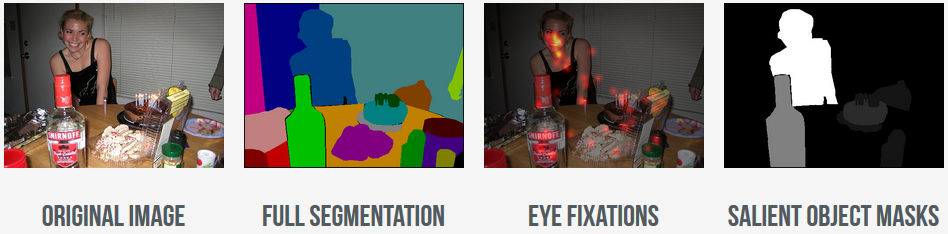
\includegraphics[width=0.95\textwidth]{fig/PASCAL-S}
\end{center}
\caption{Examples of the PASCAL-S dataset.}
\label{fig:pascal-s}
\end{figure}


The saliency segmentation method and the findings have been published at \cite{TPAMI.2012.147}.  

\subsection{Multimedia Datasets}
\subsubsection{MSRA-MM}
In 2009, the reserachers from Micsosoft Research Asia have released 2 versions of large multimedia datasets- MSRA-MM \cite{msra-mm_db}. MSRA-MM 1.0 consists of two sub-datasets, i.e., an image dataset and a video dataset that are collected from the image and video search engines. For image dataset, there are about $1000$ images per query for $68$ representative queries based on the log of search engies. There are $65443$ images in total. For the video dataset, $165$ representative queries have been selected from a log resulting in total of $10277$ videos. Due to copyright issues, the raw image and video data are not available, but only features and annotations are provided. The dataset is explained in detail in a techical report \cite{export:79942}.

\subsection{Salient Regions Datasets}
Surprisingly there are not many datasets available for testing saleint region detection.

\subsubsection{Oxford Vision Group}

For more than a decade the standart dataset was provided by Mikolajczyk et al. \cite{Mikolajczyk:2005} from the Oxford vision group. The dataset is rather small, contains only $48$ images, but real (not simulated). Illustration of the dataset can be seen on figure \ref{fig:mikdataset}. 

\begin{figure}[H]
\begin{center}
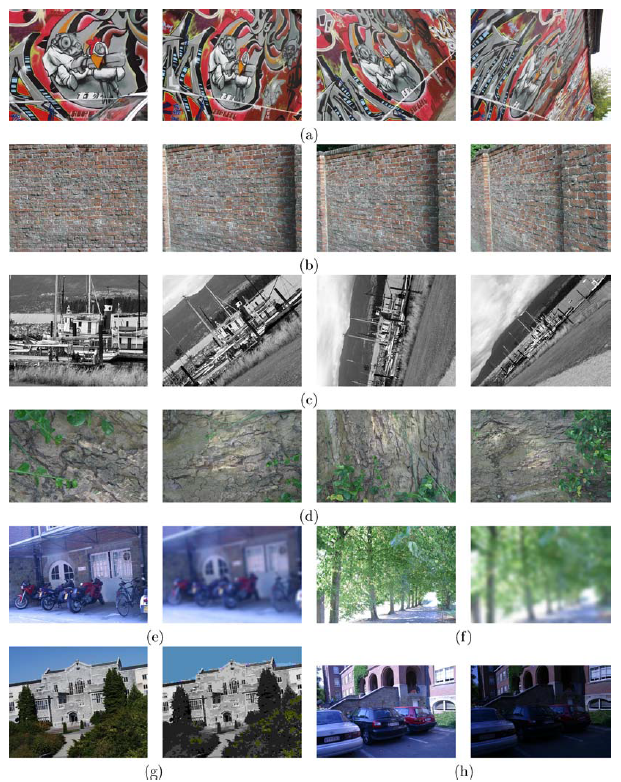
\includegraphics[width=0.95\textwidth]{fig/MikDataset}
\end{center}
\caption{Oxford vision group dataset: (a), (b) Viewpoint change, (c), (d) Zoom+rotation, (e), (f) Image blur, (g) JPEG compression, (h) Light change. In the
case of viewpoint change, scale change and blur, the same change in imaging conditions is applied to two different scene types: structured and
textured scenes. The left most image of each set is used as the reference image.}
\label{fig:mikdataset}
\end{figure}

 Five different changes in imaging conditions are represented: viewpoint changes (a) \& (b); scale changes (c) \& (d); image blur (e) \& (f); JPEG compression (g); and illumination (h). The effect of changing the image conditions can be separated from
the effect of changing the scene type. One scene type contains homogeneous regions with distinctive edge boundaries (e.g. graffiti, buildings), and the other contains
repeated textures of different forms. The authors referred to these as structured versus textured scenes respectively. For example sequence (a) is of structured type, while (b) is example of textured sequence.

In the viewpoint change test the camera varies from a fronto-parallel view to one with significant foreshortening
at approximately 60 degrees to the camera. For details of the other image transformations, the reader is referred to the publication \cite{Mikolajczyk:2005} and the data description.   All images are of small resoluton for now a days standarts, but considered medium a decade ago (approximately 800 $\times$ 640 pixels).
Since the images are either of planar scenes or the camera position is fixed during acquisition, the images are related by homographies (plane
projective transformations). All homographies between the reference (leftmost) image and the other images in a particular dataset are provided.

It is available under Test Data from \url{http://www.robots.ox.ac.uk/~vgg/research/affine/index.html}.
\subsubsection{Freiburg University}
More recently, Fissher 

\subsection{Object and Scene Recognition Datasets}
\label{subsec:obj_scene_db}

\subsubsection{MIT-CSAIL}
The goal of the MIT-CSAIL dataset \cite{mit-csail_db} is to provide a large set of images of natural scenes (principally office and street scenes), together with manual segmentations/labelings of many types of objects, so that it becomes easier to work on general multi-object detection algorithms. The dataset contains indoor and outdoor objects in officeand urban environments. There are annotations for morethan30objects in cotext in thousands of images and sequences with 2500 annotaited frames. Examples of the dataset are shown in figure \ref{fig:mit-csail}.

\begin{figure}[H]
\begin{center}
\includegraphics[width=0.95\textwidth]{fig/MIT-CSAIL}
\end{center}
\caption{Examples of the MIT-CSAIL dataset.}
\label{fig:mit-csail}
\end{figure}

\subsubsection{LabelMe}
An online annotated dataset incrementally filled up by users can be downloaded using the LabelME tool from \cite{labelme_db}. The LabelMe3D dataset contains labelled images of many everyday scenes and object categories in absolute real world 3D coordinates. The toolboxes designed to work with these datasets are described in \ref{subsec:dbannot}.

\subsubsection{SUN}
Another large dataset of annotated images covering large vaiety of scenes, places and objects within, provided also by the Computer Science and Artificial Intelligence Laboratory (CSAIL) at MIT, is the SUN dataset, \cite{sun_db}. The SUN2012 contains $16 873$ images and SUN contains currently $131067$ images, $908$ Scene categories and $4479$ object categories with more than $310k$ segmented objects. The SUN397 benchmark for scene classification can de used incuding code, precomputed features etc. The SUN dataset can bee dowloaded also with the LabelMe MATLAB Toolbox. The publication about the SUN dataset is \cite{Xiao2010}.

\subsubsection{Places}
One of the largest annotated datasets for scene recognition is the Places dataset (also by CSAIL, MIT), \cite{places_db}. It contains almost $2.5$ million images in $205$ scene categories. Along with the dataset, one can access the Places-CNNs, the convolutional neural networks trained on Places, DrawCNN- a visualization of the units' connections for the CNN, the online recognition demo and some sample MATLAB code forusing the synthetic receptive field of unit to segment image and visualize the activated regions. The pulications where the dataset is described are \cite{Zhou2014, Zhou2015}.